\textbf{R:} Para la resolución de este ejercicio, partiremos de las siguientes fórmulas:
\begin{align*}
    \hat{y}&=\arg\max_{y} P(y|x) \\
    % -
    P(y_i|x) &= \frac{count(y_i)}{P(x)} \\
    % - 
\end{align*}
Cabe mencionar que usaremos $p=2$ que es la distancia euclidiana y que se entiende que los $k$-vecinos más cercanos son los $x'$ que, para todo $x''$, cumplen 
\[ ||x-x'||_p \leq ||x-x''||_p \]

Calcularemos $||x-x'||_2$ para cada $x'$ en el conjunto de datos, entonces:
\begin{align*}
    \text{(0,0): } \sqrt{(0.2-0)^2 + (0.2-0)^2} &= \sqrt{0.08} \approx 0.28 \\
    \text{(1,0): } \sqrt{(0.2-1)^2 + (0.2-0)^2} &= \sqrt{0.68} \approx 0.82 \\
    \text{(0,1): } \sqrt{(0.2-0)^2 + (0.2-1)^2} &= \sqrt{0.68} \approx 0.82 \\
    \text{(1,1): } \sqrt{(0.2-1 )^2 + (0.2-1)^2} &= \sqrt{1.28} \approx 1.13
\end{align*}

Veamos que los $k$-vecinos más cercanos a $\mathbf{x}$ son $(0,0)$, $(1,0)$ y $(0,1)$, con clases $0$, $1$ y $0$ respectivamente. Entonces, se tiene que 
\begin{align*}
    P(y=0|x) &= \frac{2}{3} \\
    P(y=1|x) &= \frac{1}{3}
\end{align*}
Dado que al tener una mayor probabilidad para la clase $0$, se tiene que $\hat{y} = 0$, a continuacoión, se muestra una gráfica con los puntos:
\begin{center}
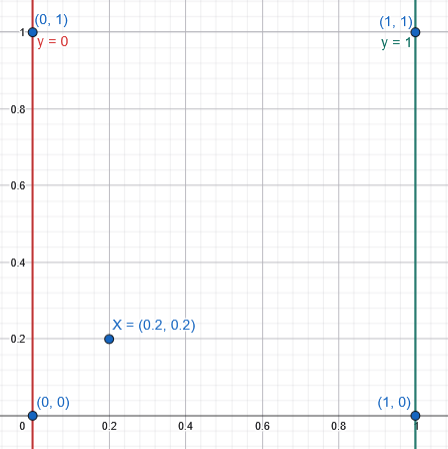
\includegraphics[height = 10cm]{ejercicios/assets/Ej4_ejemplo.png}
\end{center}